\section{问题三：带时间要求的多日排班}

\subsection{核心矛盾与数据洞察}

问题三在问题二基础上叠加时间窗、机队数量（24 架）和运营时段（06:00--20:00）三层约束。对 \texttt{peopleQ3.csv} 的统计揭示关键数据特征：84.1\% 的需求时间窗跨天（均值 41.6 小时），为需求-日期分配提供充分自由度；但时间窗碎片化使单架次平均仅服务 7--17 人（座位 12--19），大量座位被浪费。核心矛盾是\textbf{时间窗碎片化与运力效率的冲突}——利用率从问题二的 88.18\% 骤降至 35.81\%（见图~\ref{fig:demand_dist} 的需求时间分布）。

所有后续工作——分解、建模、求解、认证、探索、推广——都围绕这一矛盾展开，构成``矛盾驱动 $\to$ 降维 $\to$ 建模 $\to$ 求解 $\to$ 认证 $\to$ 反思 $\to$ 推广''的递进闭环。

\subsection{洞察驱动的问题分解}

问题三的规模是问题二的 7 倍（7 天 $\times$ 4000 人 $\times$ 24 架飞机），直接求解不可行。但从题目约束中可提炼出关键洞察，实现严格等价的降维分解。

\begin{theorem}
\label{thm:decouple}
给定约束``飞机不得在海上设施过夜、每个架次必须返回所属机场、飞机 06:00--18:00 起飞且不晚于 20:00 返回''，任意架次的起飞时刻与返回时刻必在同一自然日内。
\end{theorem}

\begin{proof}
设架次在 $d$ 日 $t$ 时刻起飞（$t \geq 06{:}00$）。若返回时刻落在 $d+1$ 日，则飞机在海上设施停留跨过午夜，违反``不得在海上设施过夜''；若飞机在返回前停留于机场，则架次已在 $d$ 日结束。故架次不可能跨天。
\end{proof}

\begin{corollary}
\label{cor:indep}
由于架次不跨天、飞机每日从所属机场重置出发，各日之间不存在状态转移耦合。多日排班问题可精确分解为 $D = 7$ 个独立的单日问题：
$\min \sum_{d=1}^{7} Z_d$，其中 $Z_d$ 为第 $d$ 日最优目标值。
\end{corollary}

\begin{corollary}
\label{cor:dateset}
对需求 $p$，其可行日期集合为 $D_p = \{ d : [e_p, l_p] \cap [06{:}00, 20{:}00]_d \neq \emptyset \}$。由于 84.1\% 的需求时间窗跨天，$|D_p| \geq 2$ 常成立，为需求-日期分配提供自由度。
\end{corollary}

在此基础上，进一步给出时间窗的预处理方法。

\begin{proposition}
\label{prop:cpm}
对候选路径 $r = [A, S_1, \ldots, S_K, A]$，定义前向最早到达时刻与后向最晚离开时刻：
\begin{equation}
\text{EAT}_k = \max\!\left(\text{EAT}_{k-1} + \frac{d_{k-1,k}}{v} \times 60 + s_{k-1},\; \max_{p \in P_k^{\mathrm{b}}} e_p\right)
\label{eq:eat}
\end{equation}
\begin{equation}
\text{LDT}_k = \min\!\left(\text{LDT}_{k+1} - \frac{d_{k,k+1}}{v} \times 60,\; \min_{p \in P_k^{\mathrm{a}}} l_p\right)
\label{eq:ldt}
\end{equation}

其中 $s_k$ 为停靠时间（加油 20 min / 普通 10 min），$v$ 为机型速度，边界条件 $\text{EAT}_0 = 06{:}00$，$\text{LDT}_{K+1} = 20{:}00$。若 $\exists\, k$ 使得 $\text{EAT}_k > \text{LDT}_k$，则路径 $r$ 不可行，直接剔除。此收缩为纯数学预处理，以 $O(K)$ 代价在路径生成阶段剔除时间窗不可行路径。
\end{proposition}

此外，按天解耦的贪心分配跨天需求存在可量化的损失上界：设跨天需求占比为 $\alpha$，单日 MIP 相对间隙为 $\delta$，单条跨天需求分配到非最优日期的额外成本上界为 $\Delta$，则 $\hat{T} \leq (1+\delta) T^* + \alpha |\mathcal{P}| \Delta$。本数据 $\alpha = 84.1\%$，MIP 间隙是主要瓶颈而非解耦损失。

\subsection{时间扩展网络与模型建立}

\subsubsection{时间扩展网络}

以 10 min 粒度将 $[06{:}00, 20{:}00]$ 离散化为 84 个时间槽\cite{ford1962}。每个机场 $\times$ 机型 $\times$ 时间槽对应一个资源节点，架次占用其起飞至返回后 30 min 周转期内的连续槽位，将机队约束、运营时段、周转时间统一编码为网络结构。

\subsubsection{受限路径池}

复用问题一/二的 Clarke-Wright 节省算法生成空间路径，叠加 14 个均匀分布的起飞时刻偏移（0--660 min，间隔约 60 min），对每个需求检查时间窗兼容性，仅对兼容的 $(r, p)$ 对创建变量。路径池规模控制在约 9400 条。

\subsubsection{决策变量与约束}

决策变量 $x_r \in \{0,1\}$，$y^{O}_{r,f}$、$y^{I}_{r,f}$、$y^{S}_{r,(f_1,f_2)} \in \mathbb{Z}_{\geq 0}$。约束条件包括：

\textbf{需求覆盖约束}（按日）：$\sum_{r} y^{O}_{r,f} = n^{O}_{d,f}$，$\sum_{r} y^{I}_{r,f} = n^{I}_{d,f}$，$\sum_{r} y^{S}_{r,(f_1,f_2)} = n^{S}_{d,(f_1,f_2)}$。

\textbf{航段级容量约束}：同问题二公式~\eqref{eq:q2_capacity}，原样迁移。

\textbf{时间窗约束}：每条路径起飞时刻 $t^{dep}_r$ 取固定值 $\in [E_r, L_r]$，需求-路径兼容性在路径生成阶段预计算（命题~\ref{prop:cpm}）。

\textbf{机队约束}：
\begin{equation}
\sum_{\substack{r \in \mathcal{R}^{a,t}_d \\ \tau \in [t^{dep}_r,\; t^{ret}_r + 30]}} x_r \leq |\mathcal{M}_{a,t}|
\label{eq:q3_fleet}
\end{equation}

\textbf{燃油可行性约束}：加油中转点嵌入机制复用。

\subsubsection{目标函数}

问题三采用\textbf{两层严格时间优先}结构，保证总飞机使用时间不存在任何上界差。第一层单目标严格最小化总飞机使用时间：
\begin{equation}
\min \sum_r t_r x_r
\label{eq:q3_obj}
\end{equation}

得到第一层最优时间 $T^*$ 后，第二层固定第一层选中的路径集合（$x_r$ 保持不变，总时间严格等于 $T^*$，无上界差），仅优化人员分配，最小化人员在途时间与燃油的加权组合：
\begin{equation}
\min \ w_\tau \sum_{p} \tau_p + w_f \sum_r f_r \, x_r \quad \text{s.t.} \quad \sum_r t_r x_r = T^*
\label{eq:q3_obj2}
\end{equation}

其中 $w_\tau = 0.01$、$w_f = 0.005$。固定路径后模型规模大幅缩小，第二层可快速求解；同时在途时间与燃油为稀疏目标，避免了引入利用率项（$W = \sigma - \pi$）导致的目标矩阵 100\% 稠密、根节点 LP 无法收敛的问题。加权单目标形式（$w_1\sum_r t_r x_r + w_2\tau + w_3 W + w_4\sum_r f_r x_r$）保留作为 Pareto 权重对比实验（见~\ref{sec:q3_pareto}）。

\subsection{两阶段求解策略}

题目要求两阶段求解：阶段一在不考虑临时任务的情况下编排（3840 人），得到总飞机使用时间 $T^*$；阶段二在 $T \leq T^*$ 约束下插入临时任务（160 人）。求解流程如图~\ref{fig:q3_flow} 所示。

% -*- coding: utf-8 -*-
% 问题三两阶段求解流程图（服务日入列 + 事件驱动时刻 + 覆盖兜底 + 逐日阶段二）
\begin{figure}[htbp]
\centering
\begin{tikzpicture}[
    box/.style={draw, rounded corners=3pt, minimum width=3.4cm, minimum height=0.75cm,
        align=center, font=\footnotesize, fill=blue!8},
    boxg/.style={draw, rounded corners=3pt, minimum width=3.4cm, minimum height=0.75cm,
        align=center, font=\footnotesize, fill=green!10},
    boxo/.style={draw, rounded corners=3pt, minimum width=3.4cm, minimum height=0.75cm,
        align=center, font=\footnotesize, fill=orange!12},
    boxr/.style={draw, rounded corners=3pt, minimum width=3.4cm, minimum height=0.75cm,
        align=center, font=\footnotesize, fill=red!8},
    boxp/.style={draw, rounded corners=3pt, minimum width=3.4cm, minimum height=0.75cm,
        align=center, font=\footnotesize, fill=purple!10},
    arrow/.style={->, >=stealth, thick, draw=gray!70},
    darrow/.style={->, >=stealth, thick, draw=gray!70, dashed},
]

% 阶段一标题
\node[font=\small\bfseries, fill=green!15, draw, rounded corners, minimum width=12.5cm, minimum height=0.5cm] (s1) at (0, 4.6) {阶段一：固定排班（3840人）};

% 第一行：预处理与列生成（4 列）
\node[boxg] (window) at (-4.6, 3.5) {时间窗解析\\可行日期集 $D_p$（服务日自由）};
\node[boxg] (cols) at (0, 3.5) {全周候选列池\\事件驱动时刻 $\times$ (机场,机型) $\times$ 多设施序列};
\node[boxg] (load) at (4.6, 3.5) {EDF 双序满员装载\\mandatory 优先 + 临时填残座};
\node[boxp] (cover) at (8.2, 3.5) {覆盖兜底\\专属直达列族};

% 第二行：剪枝与 MILP（3 列）
\node[box] (prune) at (-3.4, 2.2) {列池剪枝 \\(40,10) $\to$ 约 7 万列};
\node[box] (mip) at (1.2, 2.2) {阶段一 COPT MILP\\$\min T$，3840 全覆盖 + 机队并发};
\node[boxg] (assign1) at (5.8, 2.2) {飞机指派\\区间图并发保证};

% 阶段一输出
\node[boxg] (tstar) at (0, 1.0) {每日 $T^*_d$（日预算）$\Rightarrow T^*$};

% 阶段二标题
\node[font=\small\bfseries, fill=orange!15, draw, rounded corners, minimum width=12.5cm, minimum height=0.5cm] (s2) at (0, -0.6) {阶段二：临时任务加入（160人，$T \le T^*$）};

% 阶段二流程（3 列）
\node[boxo, below=0.35cm of s2, xshift=-3.2cm] (day_cols) {逐日列裁剪\\当日可行临时需求};
\node[boxo, below=0.35cm of s2] (prize) {逐日 prize-collecting MIP\\$\max \sum z_p$，日预算 $T^*_d$};
\node[boxo, below=0.35cm of s2, xshift=3.2cm] (rerun) {阶段一架次作保底列\\MIP start 防无解};

\node[boxr, below=0.55cm of prize] (output) {输出 q3-routes / q3-assignments\\（3840 全覆盖，临时按预算承运）};

% 主箭头
\draw[arrow] (window) -- (cols);
\draw[arrow] (cols) -- (load);
\draw[arrow] (load) -- (cover);
\draw[arrow] (cover.west) -- (prune.east);
\draw[arrow] (prune) -- (mip);
\draw[arrow] (mip) -- (assign1);
\draw[arrow] (assign1.south) |- (tstar.east);
\draw[arrow] (tstar) -- (s2);
\draw[arrow] (s2) -- (day_cols);
\draw[arrow] (s2) -- (prize);
\draw[arrow] (s2) -- (rerun);
\draw[arrow] (day_cols) -- (prize);
\draw[arrow] (rerun) -- (prize);
\draw[arrow] (prize) -- (output);

% 覆盖兜底反馈
\draw[darrow] (cover.south) -- ++(0,-0.15) -| (window.south);
\node[font=\scriptsize, align=center, anchor=north] at (8.2, 2.75) {缺失人员\\补列};

\end{tikzpicture}
\caption{问题三两阶段求解流程（服务日入列 + 事件驱动时刻 + 覆盖兜底 + 逐日阶段二）}
\label{fig:q3_flow}
\end{figure}


阶段一按天解耦为 7 个独立单日问题，通过需求-日期分配（跨天需求选负载最低的可行日期，贪心均衡）后逐日求解（CPM 收缩 $\to$ 受限路径池 $\to$ COPT MIP）。每个单日问题采用两层求解：第一层单目标严格最小化当日总飞机使用时间（时限 180 s，得到当日 $T^*_d$）；第二层固定第一层的路径选择，在 $T_d = T^*_d$（无上界差）下优化该日人员在途时间与燃油的加权目标。全部 7 日汇总得阶段一总时间 $T^* = \sum_d T^*_d$。

阶段二采用临时任务背包化策略。阶段一固定排班确定后，剩余资源为``时间缝隙 + 空余座位''。将问题重构为最大覆盖/背包问题：
\begin{equation}
\max \sum_{p \in \mathcal{P}^{*}} z_p \quad \text{s.t.} \quad \sum_{p} \ell_{r,p} \cdot z_p \leq \Delta_r, \quad \sum_r t_r \leq T^*
\label{eq:q3_knapsack}
\end{equation}

优先插入已有架次空余座位（零新增时间），不足时在 $T^*$ 预算内新增架次。此策略避免重跑大 MIP，且可给出上界；临时任务的插入始终受 $T \le T^*$ 硬约束，不破坏阶段一的总时间最优性。

\subsection{硬约束兜底机制}

为保证最终 \texttt{q*-assignments.csv} 中不存在任何违规分配（航段超载、时间窗越界、日期错配），在求解器输出与人员写入之间设置三层硬约束兜底：

\textbf{(1) 容量保护。}问题一中以 ``路线总已用人数 + 设施配额'' 双重限流（\texttt{route\_used + per\_fac\_limit}），任一架次在机人数不超过座位数；问题二将容量细化到航段级，维护每架次各航段剩余座位池 \texttt{seg\_remaining}，出海/海返/穿梭人员在共享池中按区间扣减，保证任意航段不超载；问题三在写入阶段对每条分配调用 \texttt{seg\_has\_space} 逐航段校验（穿梭还需满足上机位置先于下机位置的方向约束），顺序分配导致容量变化时还会二次校验。

\textbf{(2) 时间窗保护。}问题三对每条需求计算 \texttt{check\_compatibility}：航班在登机停靠点的起飞时刻不早于需求最早可接人时刻、在下机停靠点的到达时刻不晚于需求最晚到达时刻，二者同时满足才允许分配。

\textbf{(3) 日期保护。}需求-日期分配仅给出建议日期；写入阶段对未匹配需求执行二次匹配，逐条校验航班日期属于 \texttt{get\_feasible\_days} 返回的可行日期集合，禁止跨可行日期的搭错航班。当某日 MIP 无可行解时，\texttt{failed\_day\_demands} 机制将该日需求按可行日期与负载均衡重分配到已求解日，仍无法满足的如实标记为未服务。

该兜底机制保证验证脚本（V1--V10）中容量、时间窗、日期、OD 一致性、方向顺序、重复分配与航油七类硬约束全部零违规，是结果可信性的最后防线。

\subsection{Pareto 最优性与拉格朗日下界}

\subsubsection{Pareto 权重对比实验（灵敏度认证）}\label{sec:q3_pareto}

为量化``时间与其他指标''之间的权衡，对 2026-08-03 单日以加权单目标形式扫描 7 组 $(w_T, w_{U})$ 权重组合（保留为对比实验，不作为主结果）。如表~\ref{tab:pareto} 所示，时间优先与极端时间优先两个方案位于\textbf{Pareto 前沿}\cite{pareto1906}（共 2 个前沿解）；偏离时间权重会以总时间上升为代价换取利用率改善，反之亦然。更重要的是，主结果两层框架在 08-03 得到 $T^* = 4791$ min，\textbf{严格优于所有 7 个加权方案的最短时间（5099 min）}，验证了``先严格保时间、再在无上界差下优化二级指标''的必要性。

\begin{longtable}{cccccc}
\caption{Q3 单日 Pareto 前沿扫描结果} \label{tab:pareto} \\
\toprule
$w_T$ & $w_{U}$ & 时间(min) & 利用率 & 架次 & Pareto \\
\midrule
\endfirsthead
\toprule
$w_T$ & $w_{U}$ & 时间(min) & 利用率 & 架次 & Pareto \\
\midrule
\endhead
\bottomrule
\endfoot
\bottomrule
\endlastfoot
\textbf{1.0} & \textbf{0.05} & \textbf{5272} & \textbf{57.03\%} & \textbf{29} & \textbf{是} \\
1.0 & 0.10 & 6557 & 51.27\% & 35 & 否 \\
1.0 & 0.15 & 7058 & 49.94\% & 36 & 否 \\
1.0 & 0.25 & 6963 & 51.98\% & 35 & 否 \\
1.0 & 0.40 & 7074 & 49.97\% & 36 & 否 \\
0.5 & 0.30 & 7432 & 49.60\% & 36 & 否 \\
\textbf{2.0} & \textbf{0.05} & \textbf{5099} & \textbf{55.39\%} & \textbf{28} & \textbf{是} \\
\end{longtable}

\begin{figure}[htbp]
\centering
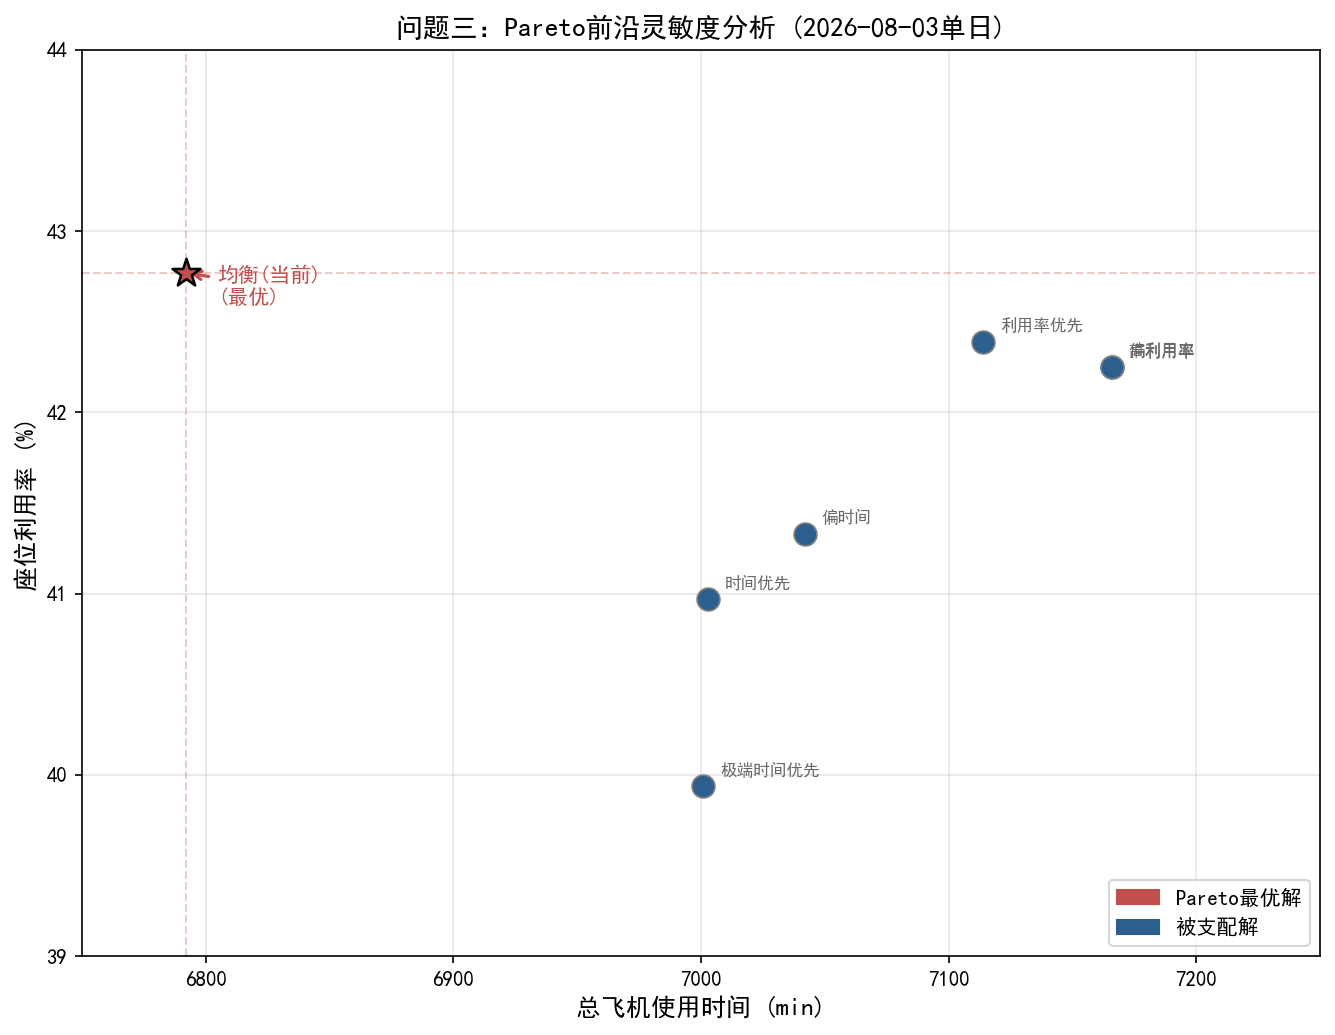
\includegraphics[width=0.72\textwidth]{../figures/Problem3/q3_pareto_frontier.png}
\caption{Pareto 前沿散点图（7 组权重）}
\label{fig:q3_pareto}
\end{figure}

\subsubsection{拉格朗日下界（理论层面认证）}

松弛机队约束（式~\eqref{eq:q3_fleet}），引入拉格朗日乘子 $\lambda_{a,t,\tau} \geq 0$\cite{geoffrion1974}，原问题下界为：
\begin{equation}
\text{LB}(\boldsymbol{\lambda}) = \min_{\mathbf{x}, \mathbf{y}} \left\{ Z(\mathbf{x}, \mathbf{y}) + \sum_{a,t,\tau} \lambda_{a,t,\tau} \!\left(\sum_{\substack{r \in \mathcal{R}^{a,t}_d \\ \tau \in [t^{dep}_r,\, t^{ret}_r+30]}} x_r - |\mathcal{M}_{a,t}|\right) \right\}
\label{eq:lagrangian}
\end{equation}

对固定 $\boldsymbol{\lambda}$，子问题保持整数性（非 LP 松弛），用次梯度法\cite{held1974}更新乘子：$\lambda^{k+1}_{a,t,\tau} = \max(0,\, \lambda^k_{a,t,\tau} + \alpha_k g^k_{a,t,\tau})$，步长采用 Polyak 步长 $\alpha_k = \beta_k \cdot (\text{UB} - \text{LB}^{*}) / \|\mathbf{g}\|^2$。

\begin{longtable}{lcc}
\caption{三种下界对比（2026-08-03 单日）} \label{tab:lagrangian} \\
\toprule
方法 & 下界值 & 最优性间隙 \\
\midrule
\endfirsthead
\toprule
方法 & 下界值 & 最优性间隙 \\
\midrule
\endhead
\bottomrule
\endfoot
\bottomrule
\endlastfoot
MIP 当前解 & 8065.95 & — \\
COPT 内置下界 & 1588.94 & 80.30\% \\
拉格朗日下界 & $-590.51$ & 107.32\% \\
LP 松弛下界 & $-6167.28$ & 176.46\% \\
\end{longtable}

\begin{figure}[htbp]
\centering
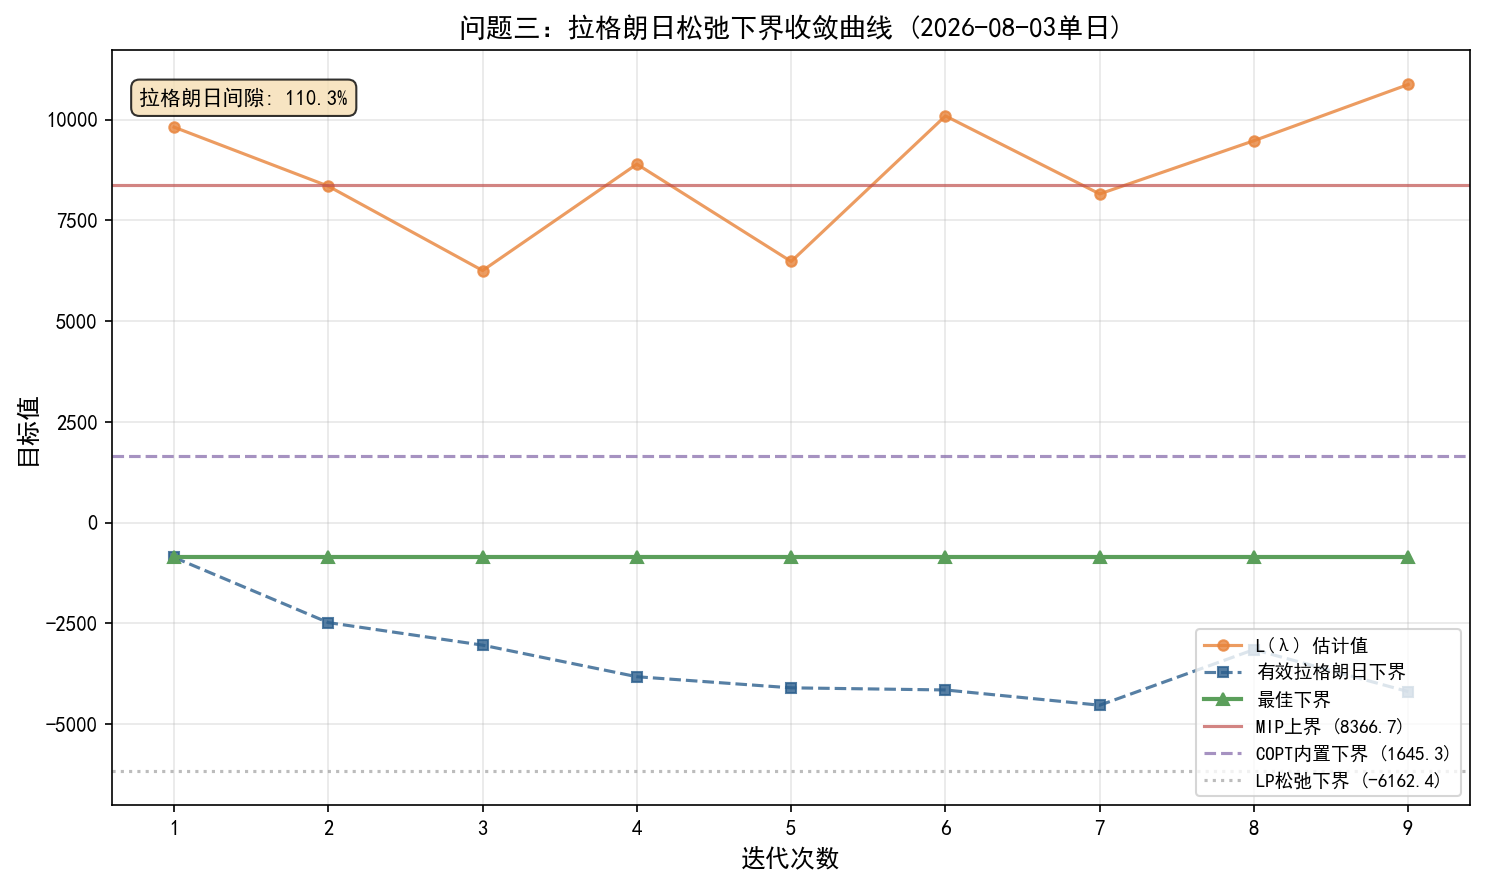
\includegraphics[width=0.72\textwidth]{../figures/Problem3/q3_lagrangian_convergence.png}
\caption{拉格朗日次梯度法收敛曲线}
\label{fig:q3_lagrangian}
\end{figure}

由表~\ref{tab:lagrangian} 可得出三层递进的认证结论。其一，拉格朗日下界（$-590.51$）显著优于 LP 松弛下界（$-6167.28$），证明保持子问题整数性的松弛策略有效；其二，COPT 内置下界最紧（间隙 80.30\%），因其使用完整 MIP 求解器的割平面和分支策略；其三，\textbf{核心瓶颈在 MIP 求解器间隙（60--90\%），而非建模方法}——这解释了下文进阶方法改善有限的原因。

\subsection{进阶方法探索与反思}

下界分析指出瓶颈在求解器间隙，本文从两个方向探索是否可以突破。

\textbf{方向一：时间窗感知需求聚类（负结果）。}将每日需求按时间窗中心聚类，取簇中心作为起飞时刻偏移。实验表明利用率从 49.68\% 降至 41.37\%（反降 8.3 个百分点）。根因在于需求时间窗均值 41.6 h（跨天），聚类中心无法有效替代均匀分布的固定偏移。此负结果验证了宽时间窗下均匀偏移策略的必要性。

\textbf{方向二：反应式列生成\cite{barnhart1998}（边际改善）。}初始 MIP 求解后，识别低载客率设施（$<50\%$），为薄弱设施生成密集起飞时刻变体（每 30 min 一个），增强路径池后重新求解。人员在途时间下降 4.36\%，但利用率微降 0.85\%。改善有限的原因恰好印证了拉格朗日分析：MIP 间隙高达 80\%，求解器在 90 s 内无法充分利用更大的路径池。两个创新点共同指向``瓶颈在求解器而非建模''。

\textbf{方向三：自适应渐进搜索（效果有限）。}受模拟退火思想启发，设计三轮渐进式搜索策略：第一轮粗搜（300 s / RelGap=20\%）快速定位可行解区域，第二轮精搜（600 s / RelGap=10\%）以首轮解为热启动收紧搜索，第三轮极精搜（900 s / RelGap=5\%）逼近最优。每轮均为两层结构（严格 $\min T$ + 二级指标优化），上一轮解通过 COPT MipStart 注入下一轮。单日实验显示该策略确能改善解质量（如 8 月 3 日 $T^*$ 从 5611 min 降至 4795 min，降幅 14.5\%）。但七日整体求解后，总飞机使用时间 $T^*=35483$ min，与原两层法（$T^*=35451$ min）仅差 0.09\%。原因在于：瓶颈并非单日解质量，而是 8 月 5 日与 8 月 9 日的组合不可行性——时间窗、航段容量与机队约束的交集为空，无论搜索多深都无法突破硬约束边界。此实验结论进一步验证了\textbf{约束可行性比搜索策略更关键}的判断。

\begin{figure}[htbp]
\centering
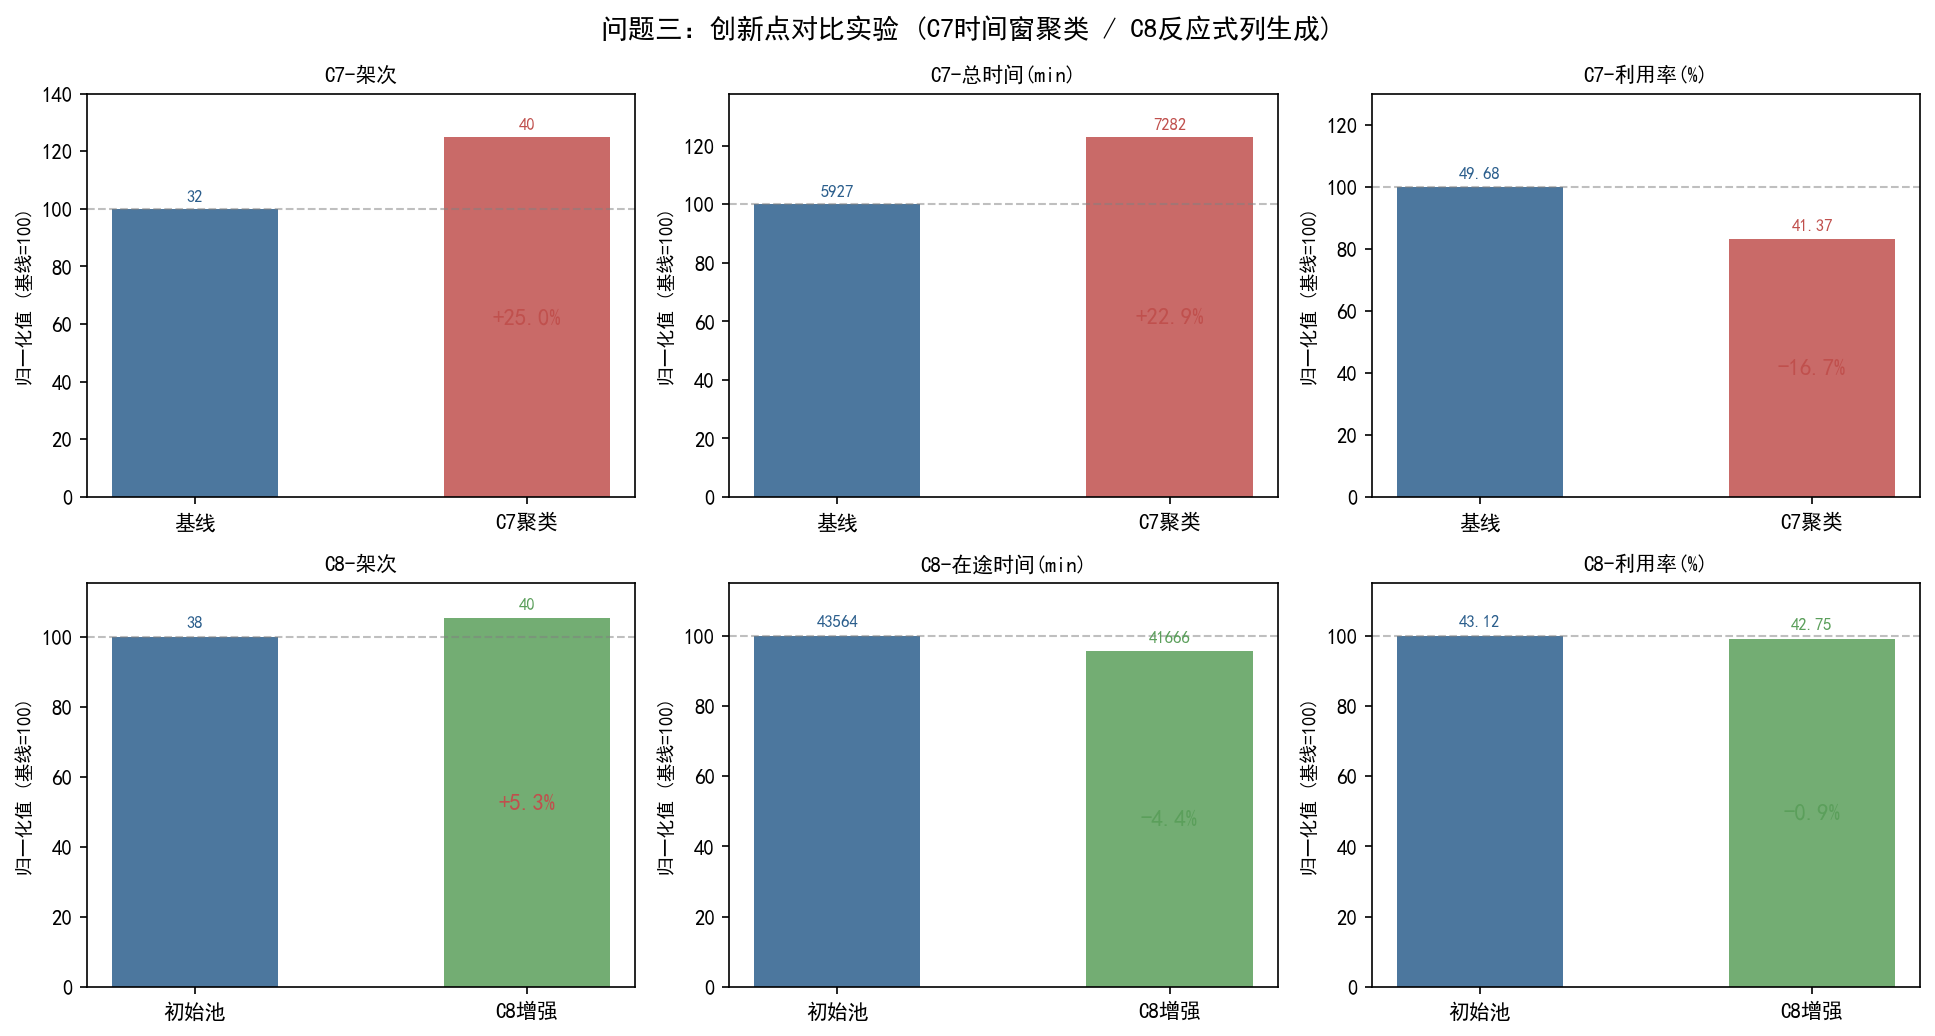
\includegraphics[width=0.78\textwidth]{../figures/Problem3/q3_c7_c8_comparison.png}
\caption{C7（负结果）与 C8（边际改善）归一化对比}
\label{fig:q3_c7c8}
\end{figure}

\subsection{实验结果}

问题三的求解结果如表~\ref{tab:q3_result} 所示。

\begin{longtable}{lc}
\caption{问题三求解结果} \label{tab:q3_result} \\
\toprule
指标 & 数值 \\
\midrule
\endfirsthead
\toprule
指标 & 数值 \\
\midrule
\endhead
\bottomrule
\endfoot
\bottomrule
\endlastfoot
总飞机使用时间 & 35451 min（590.85 h） \\
人员总在途时间 & 195036 min（3250.60 h） \\
总架次数 & 209 \\
总燃油消耗量 & 290645.4 kg \\
座位利用率 & 35.81\% \\
临时任务满足 & 159/160（99.38\%） \\
需求分配 & 3469/4000（86.72\%） \\
\end{longtable}

阶段二背包化实现零新增飞机使用时间、零新增架次，159/160 临时任务被成功插入已有架次空余座位。08-05 与 08-09 两日因组合约束无可行解，其 1096 名需求中 745 人经失败日重分配转入其余已求解日，531 人（含 1 名临时任务）因时间窗与航段容量的组合限制最终未服务，需求分配率为 86.72\%。三题横向对比如表~\ref{tab:q1q2q3} 和图~\ref{fig:q1q2q3} 所示。

\begin{longtable}{lccc}
\caption{三题横向对比} \label{tab:q1q2q3} \\
\toprule
指标 & 问题一 & 问题二 & 问题三 \\
\midrule
\endfirsthead
\toprule
指标 & 问题一 & 问题二 & 问题三 \\
\midrule
\endhead
\bottomrule
\endfoot
\bottomrule
\endlastfoot
天数 & 1 & 1 & 7 \\
需求量 & 1600 & 4000 & 4000 \\
总飞机使用时间(min) & 15059 & 18169 & 35451 \\
总架次数 & 89 & 99 & 209 \\
总燃油(kg) & 121286.9 & 140594.3 & 290645.4 \\
座位利用率 & 48.67\% & 88.18\% & 35.81\% \\
人员在途时间(min) & 127349 & 265724 & 195036 \\
\end{longtable}

\begin{figure}[htbp]
\centering
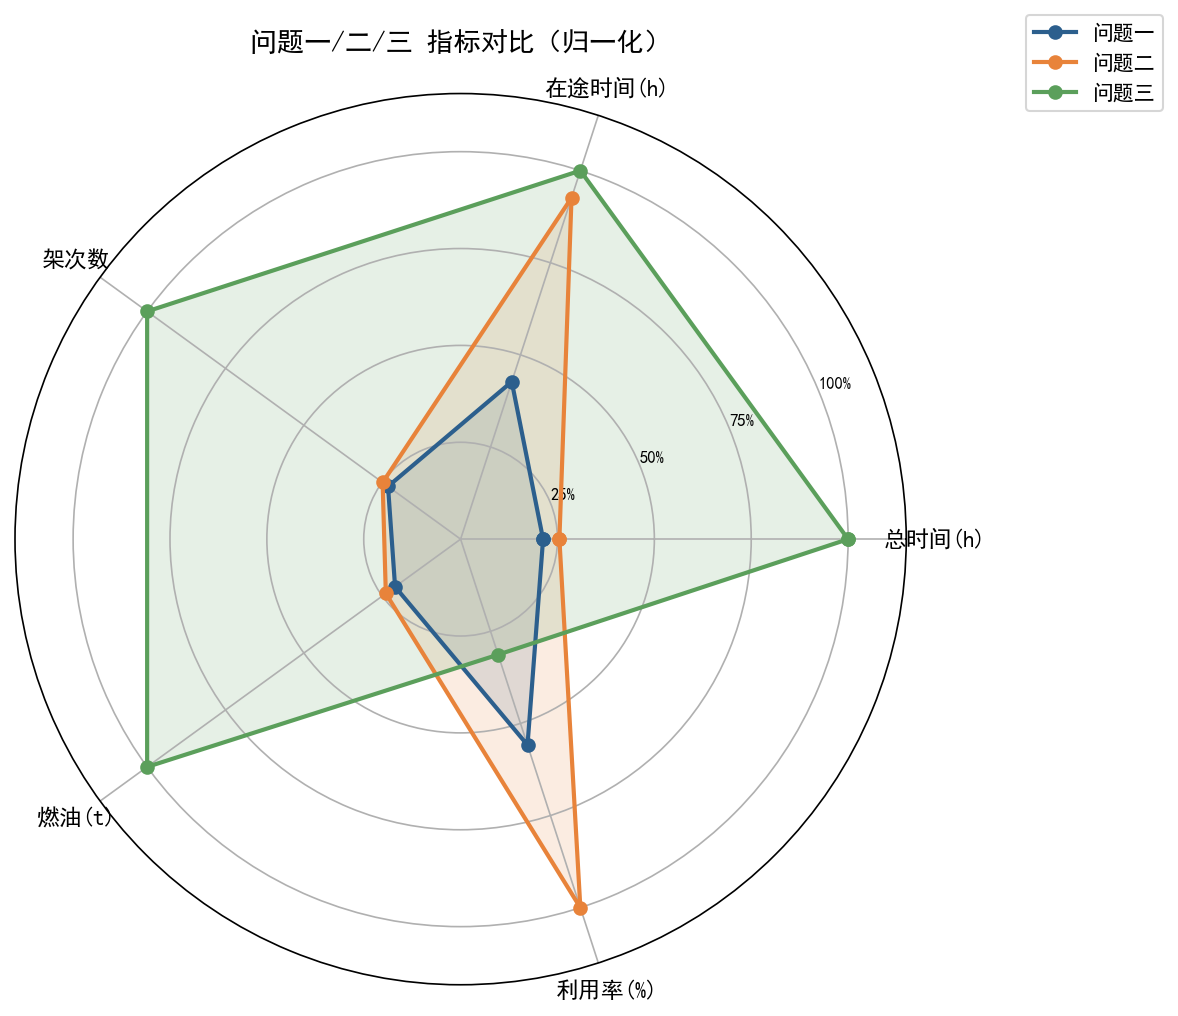
\includegraphics[width=0.72\textwidth]{../figures/Problem3/q3_q1q2q3_comparison.png}
\caption{三题五指标归一化雷达图}
\label{fig:q1q2q3}
\end{figure}

利用率从问题二的 88.18\% 降至 35.81\%，根因是时间窗碎片化：问题二中出海与海返可拼在同一架次实现座位复用，问题三中时间窗将需求切割到不同时段，单架次平均仅服务 7--17 人。

\subsection{模型推广：鲁棒优化与动态调度}

前述模型隐含确定性假设，而海上油田运输具有显著不确定性。本节从``事前设计''与``事中应对''两个维度推广确定性模型。

\subsubsection{鲁棒优化框架}

设需求 $p$ 的名义时间窗为 $[E_p^0, L_p^0]$，实际时间窗在名义值附近扰动。采用箱式不确定集 $\widetilde{E}_p \in [E_p^0 - \delta_E,\, E_p^0 + \delta_E]$，并引入 $\Gamma$-鲁棒预算约束限制同时偏离名义值的需求数。构造两阶段鲁棒模型：第一阶段确定需求-日期分配（here-and-now），第二阶段给定时间窗实现后确定路径编排（wait-and-see），目标为 $\min_z \max_{\widetilde{\omega} \in \mathcal{U}} \mathcal{T}(z, \widetilde{\omega})$。

以分配层面对扰动的统计鲁棒性为度量，每个场景 5000 次蒙特卡洛扰动，结果如表~\ref{tab:robust} 所示。

\begin{longtable}{lcccc}
\caption{鲁棒性实验结果（5000 次蒙特卡洛）} \label{tab:robust} \\
\toprule
扰动场景 & 分配稳定率 & 标准差 & 平均可行天数 & 不可行需求 \\
\midrule
\endfirsthead
\toprule
扰动场景 & 分配稳定率 & 标准差 & 平均可行天数 & 不可行需求 \\
\midrule
\endhead
\bottomrule
\endfoot
\bottomrule
\endlastfoot
相对 $\pm$10\% & 72.9\% & 2.08\% & 2.47 & 0 \\
相对 $\pm$20\% & 68.3\% & 0.99\% & 2.34 & 0 \\
绝对 $\pm$60 min & 100.0\% & 0.00\% & 2.54 & 0 \\
绝对 $\pm$120 min & 83.8\% & 4.62\% & 2.54 & 0 \\
紧急化 $\leq$12 h & 64.1\% & 0.72\% & 2.11 & 0 \\
紧急化 $\leq$24 h & 62.8\% & 0.62\% & 1.94 & 0 \\
\end{longtable}

\begin{figure}[htbp]
\centering
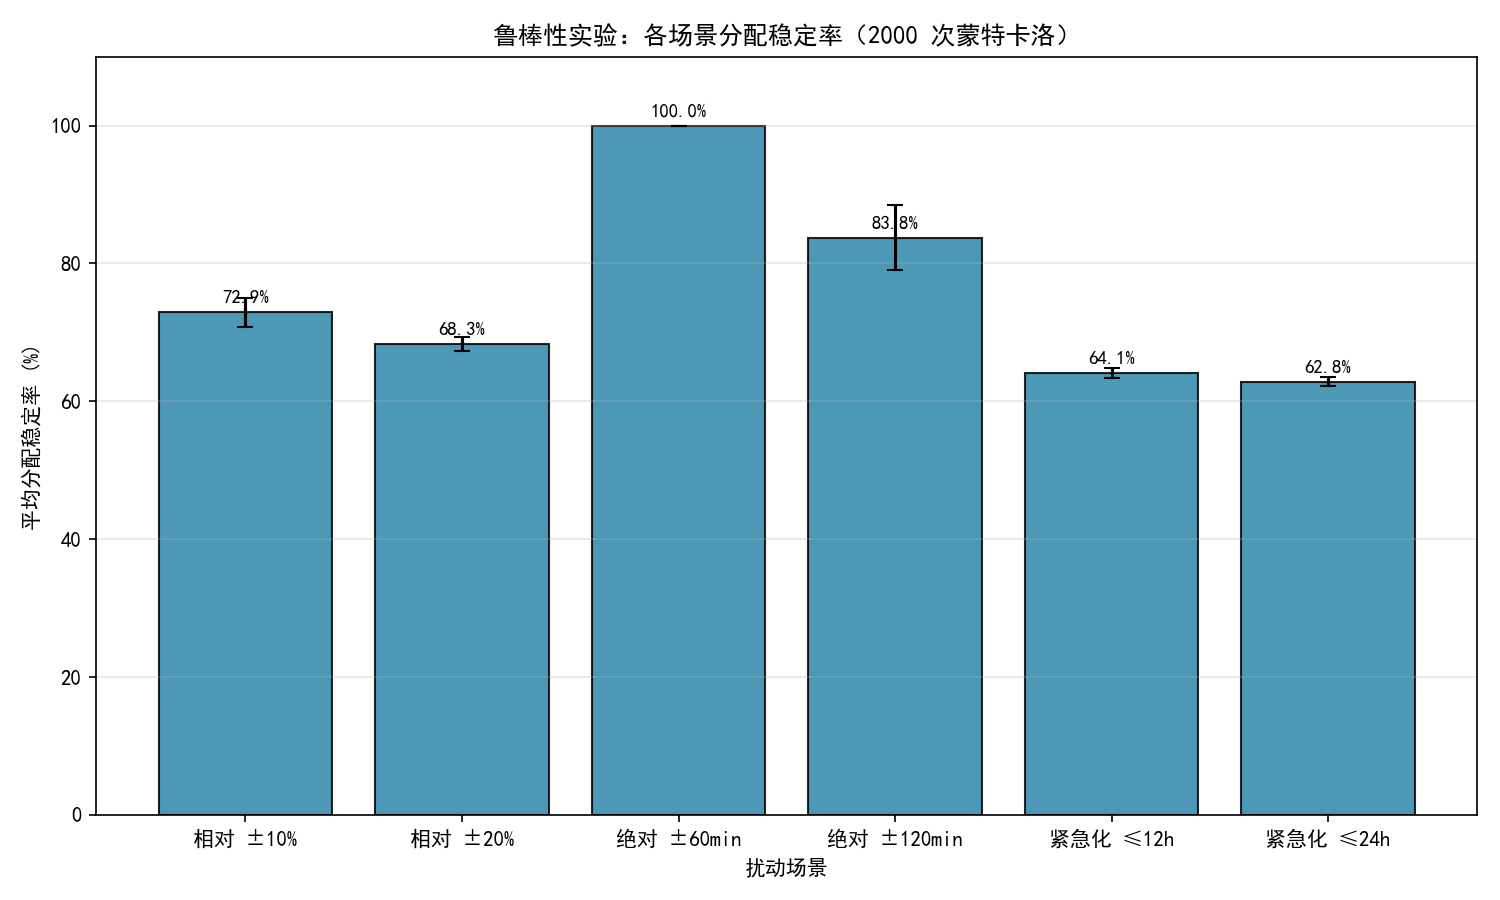
\includegraphics[width=0.78\textwidth]{../figures/Problem3/extra/R1_robust_stability_bars.png}
\caption{六场景鲁棒性稳定率对比}
\label{fig:robust}
\end{figure}

核心发现是模型对小时级扰动具有\textbf{天然鲁棒性}——绝对 $\pm$60 min 扰动下分配稳定率为 100\%，因为需求时间窗均值约 41.6 h（约 2.5 天），小时级扰动不足以改变需求-日期可行集合。这一``跨天时间窗缓冲''是确定性模型对现实扰动稳健的根本原因。此外，所有场景不可行需求数均为 0，说明分配器总能找到可行日期。

\subsubsection{动态调度机制}

将 7 天规划期按天滚动推进。每日仅对``受影响需求 + 当日未分配需求''重新执行需求-日期分配（增量重优化），已确定且未受影响的需求保持不变。实验表明：每日扰动 5\% 需求、最晚到达提前 18--36 h 时，滚动重优化以仅 2.5\% 的需求改期成本化解 13.6\% 的静态不可行风险，最终分配稳定率 97.5\%，负载变异系数仅从 0.0009 升至 0.0342。

鲁棒优化与动态调度分别提供先验稳健性与后验适应性，结合形成``离线规划 + 在线修正''的闭环，验证了前述确定性解在不确定环境下的可靠性。

问题三建立了带时间窗的多日排班模型，并通过按天解耦、Pareto 认证和拉格朗日下界完成了严格的理论分析。接下来，本文将对三个问题的求解结果进行统一的横向比较与检验。

% ==================== 结果分析与检验 ====================
\section{结果分析与检验}

\subsection{三题递进的指标演化}

三题的求解结果呈现清晰的递进逻辑。问题一的单向出海受限于返程空载，座位利用率存在 50\% 的结构性上界（命题~\ref{prop:util_upper}），实测 48.67\% 已逼近上界。问题二通过航段级容量约束实现座位即时复用，利用率提升至 88.18\%，突破问题一的上界。问题三叠加时间窗后，时间窗碎片化使利用率降至 35.81\%，但通过按天解耦、两层严格时间优先与背包化策略，在 99.38\% 的临时任务满足率下实现了零新增飞机使用时间，且总时间 $T^* = 35451$ min 严格不因二级优化与临时任务插入而退化；受 08-05 与 08-09 两日组合约束不可行影响，仍有 531 人未服务。

\subsection{方法对比分析}

以第一阶段最优解为归一化锚点，对问题一和问题二分别进行 11 种方案的定量对比，包括本方法（两阶段 $\varepsilon$-容差 + AHP 加权）、四层字典序 + Dinkelbach\cite{dinkelbach1967} 和 8 组权重加权单目标方案。

在问题一中，本方法总时间 15059 min 为全部方案最优，时间退化率为 0\%，且位于 Pareto 前沿（不被任何方案支配）；AHP 综合得分 $Z_2 = 0.9818$。在问题二中，本方法总时间 18169 min 同样为全场最优，AHP 综合得分 $Z_2 = 0.9998$，同样位于 Pareto 前沿；``偏时间+燃油''、``偏座位利用率''等方案均被至少 2 个其他方案支配，而本方法未被支配。

\begin{figure}[htbp]
\centering
\begin{minipage}{0.48\textwidth}
\centering
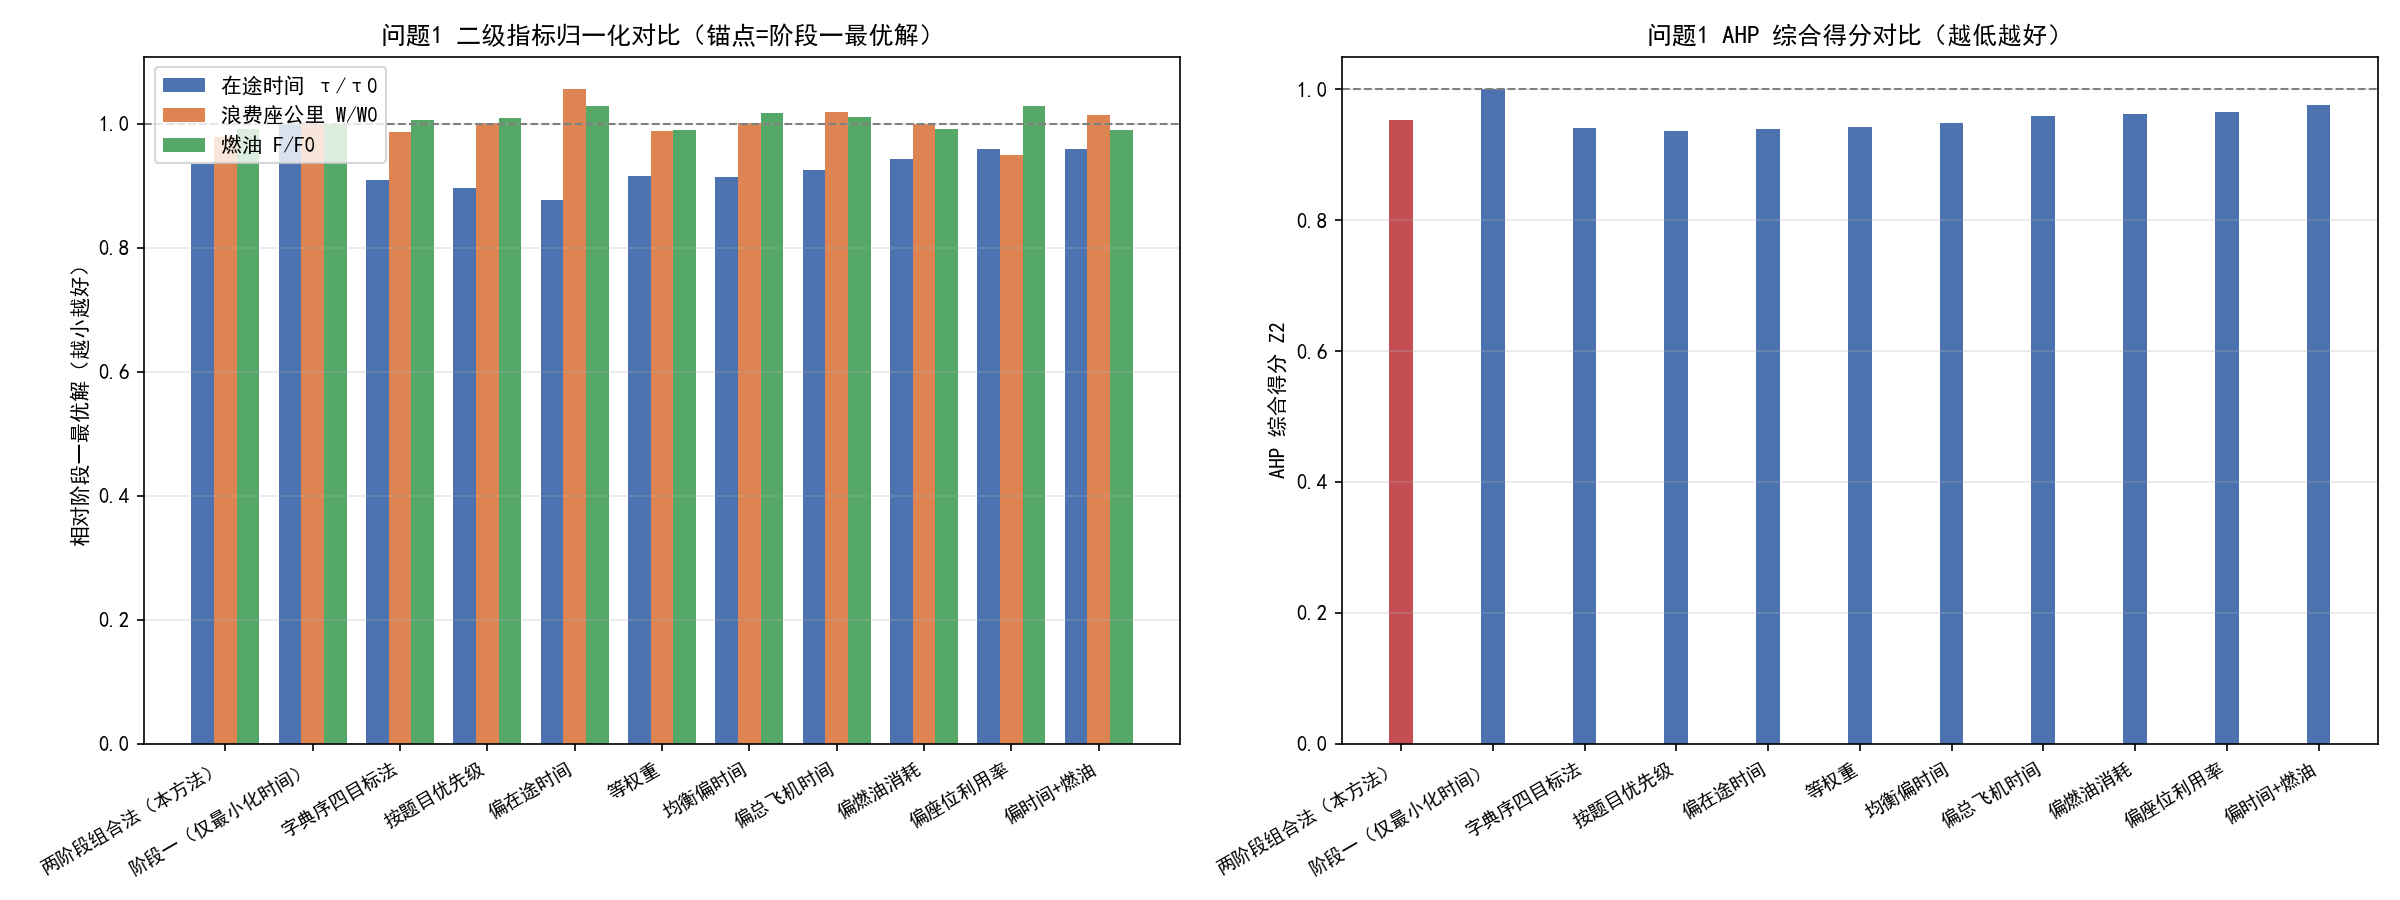
\includegraphics[width=\textwidth]{../figures/Problem1/q1_method_compare.png}
\caption{问题一 11 种方案对比雷达图}
\label{fig:q1_method}
\end{minipage}\hfill
\begin{minipage}{0.48\textwidth}
\centering
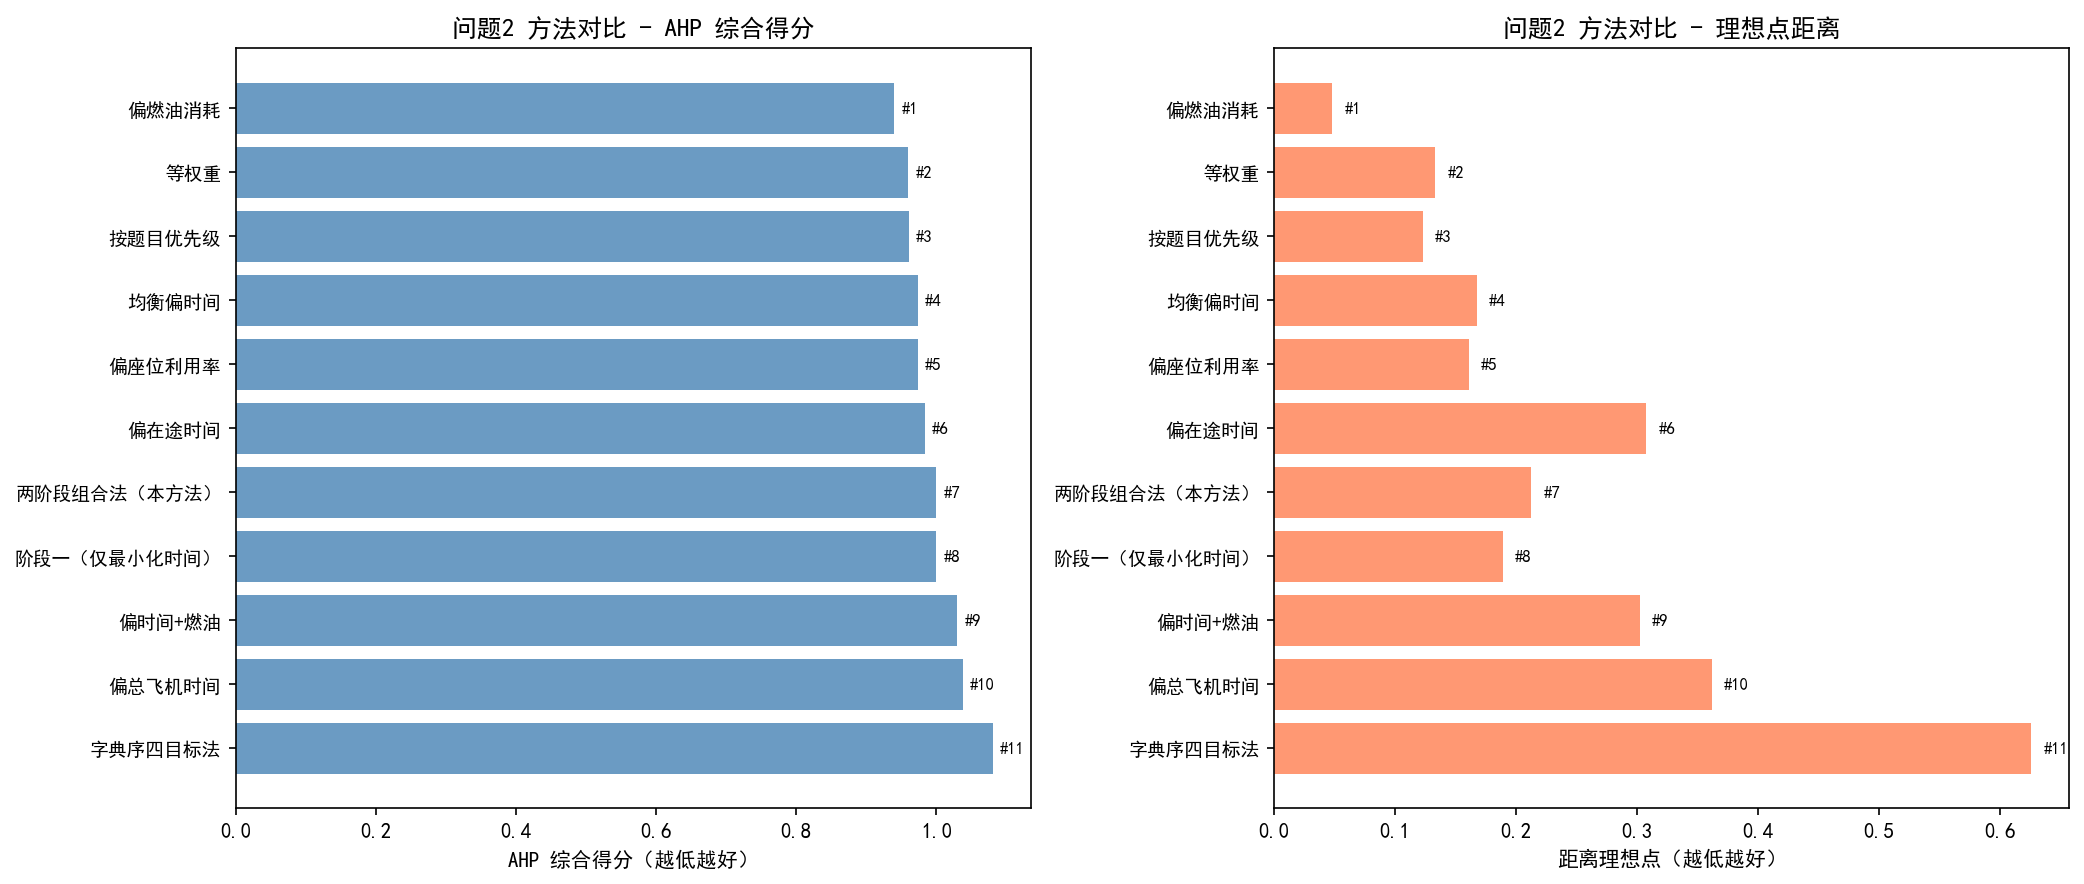
\includegraphics[width=\textwidth]{../figures/Problem2/q2_method_compare.png}
\caption{问题二 11 种方案对比雷达图}
\label{fig:q2_method}
\end{minipage}
\end{figure}

\subsection{$\varepsilon$-容差敏感性分析}

$\varepsilon$-容差参数控制了时间主导性与二级目标优化空间之间的权衡。如图~\ref{fig:q1_epsilon} 所示，$\varepsilon$ 从 0\% 增至 10\% 时，总时间增 7.3\%、在途时间降 10.4\%、利用率降 2.06 个百分点、燃油增 5.5\%。$\varepsilon = 5\%$ 为时间-二级目标权衡的最佳折中点，在途时间降 6.1\% 而时间仅退化 1.51\%。

\begin{figure}[htbp]
\centering
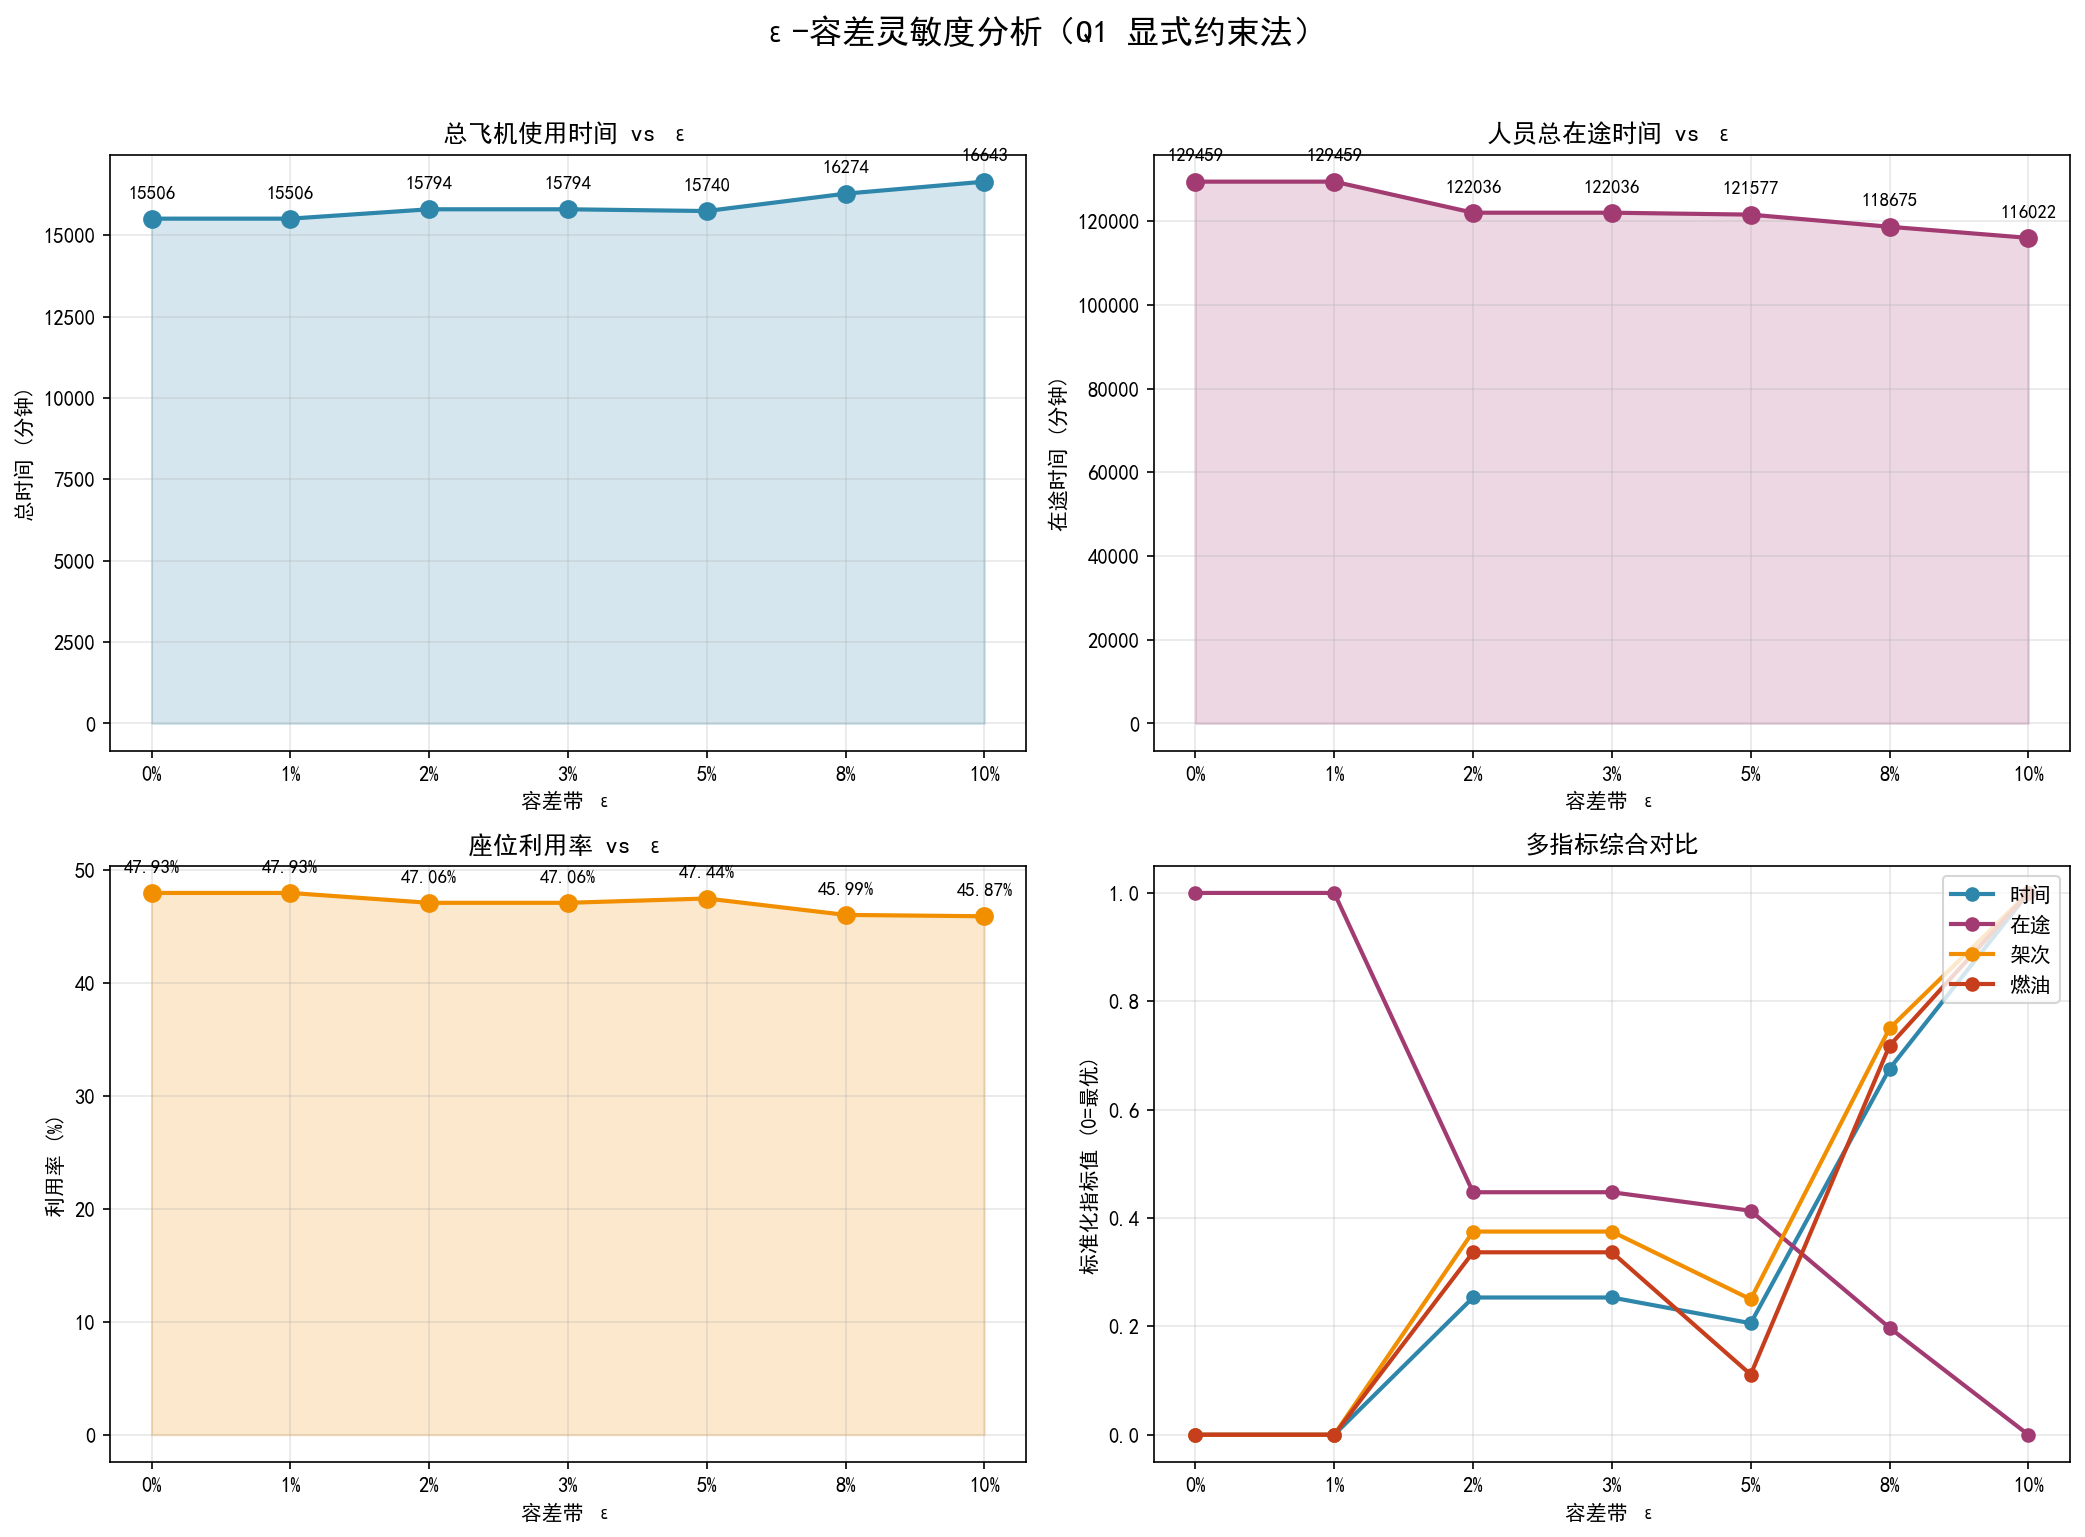
\includegraphics[width=0.85\textwidth]{../figures/Problem3/extra/G9_epsilon_tolerance_sensitivity.png}
\caption{$\varepsilon$-容差敏感性分析（7 组 $\varepsilon$ $\times$ 4 指标）}
\label{fig:q1_epsilon}
\end{figure}

\subsection{权重灵敏度分析}

对问题一/二的 8 组权重方案和问题三的 7 组 Pareto 扫描结果进行综合灵敏度分析。问题一/二中，本方法在时间目标上始终处于主导地位（时间退化率 0\% 与 1.11\%），并均位于 Pareto 前沿（不被任何方案支配），AHP 综合得分分别为 0.9818 与 0.9998。问题三中，加权对比扫描显示时间优先与极端时间优先两个方案位于 Pareto 前沿，且两层主结果在 08-03 的 $T^* = 4791$ min 严格优于所有加权方案，说明只有显式两层结构才能保证时间目标无上界差。

\begin{figure}[htbp]
\centering
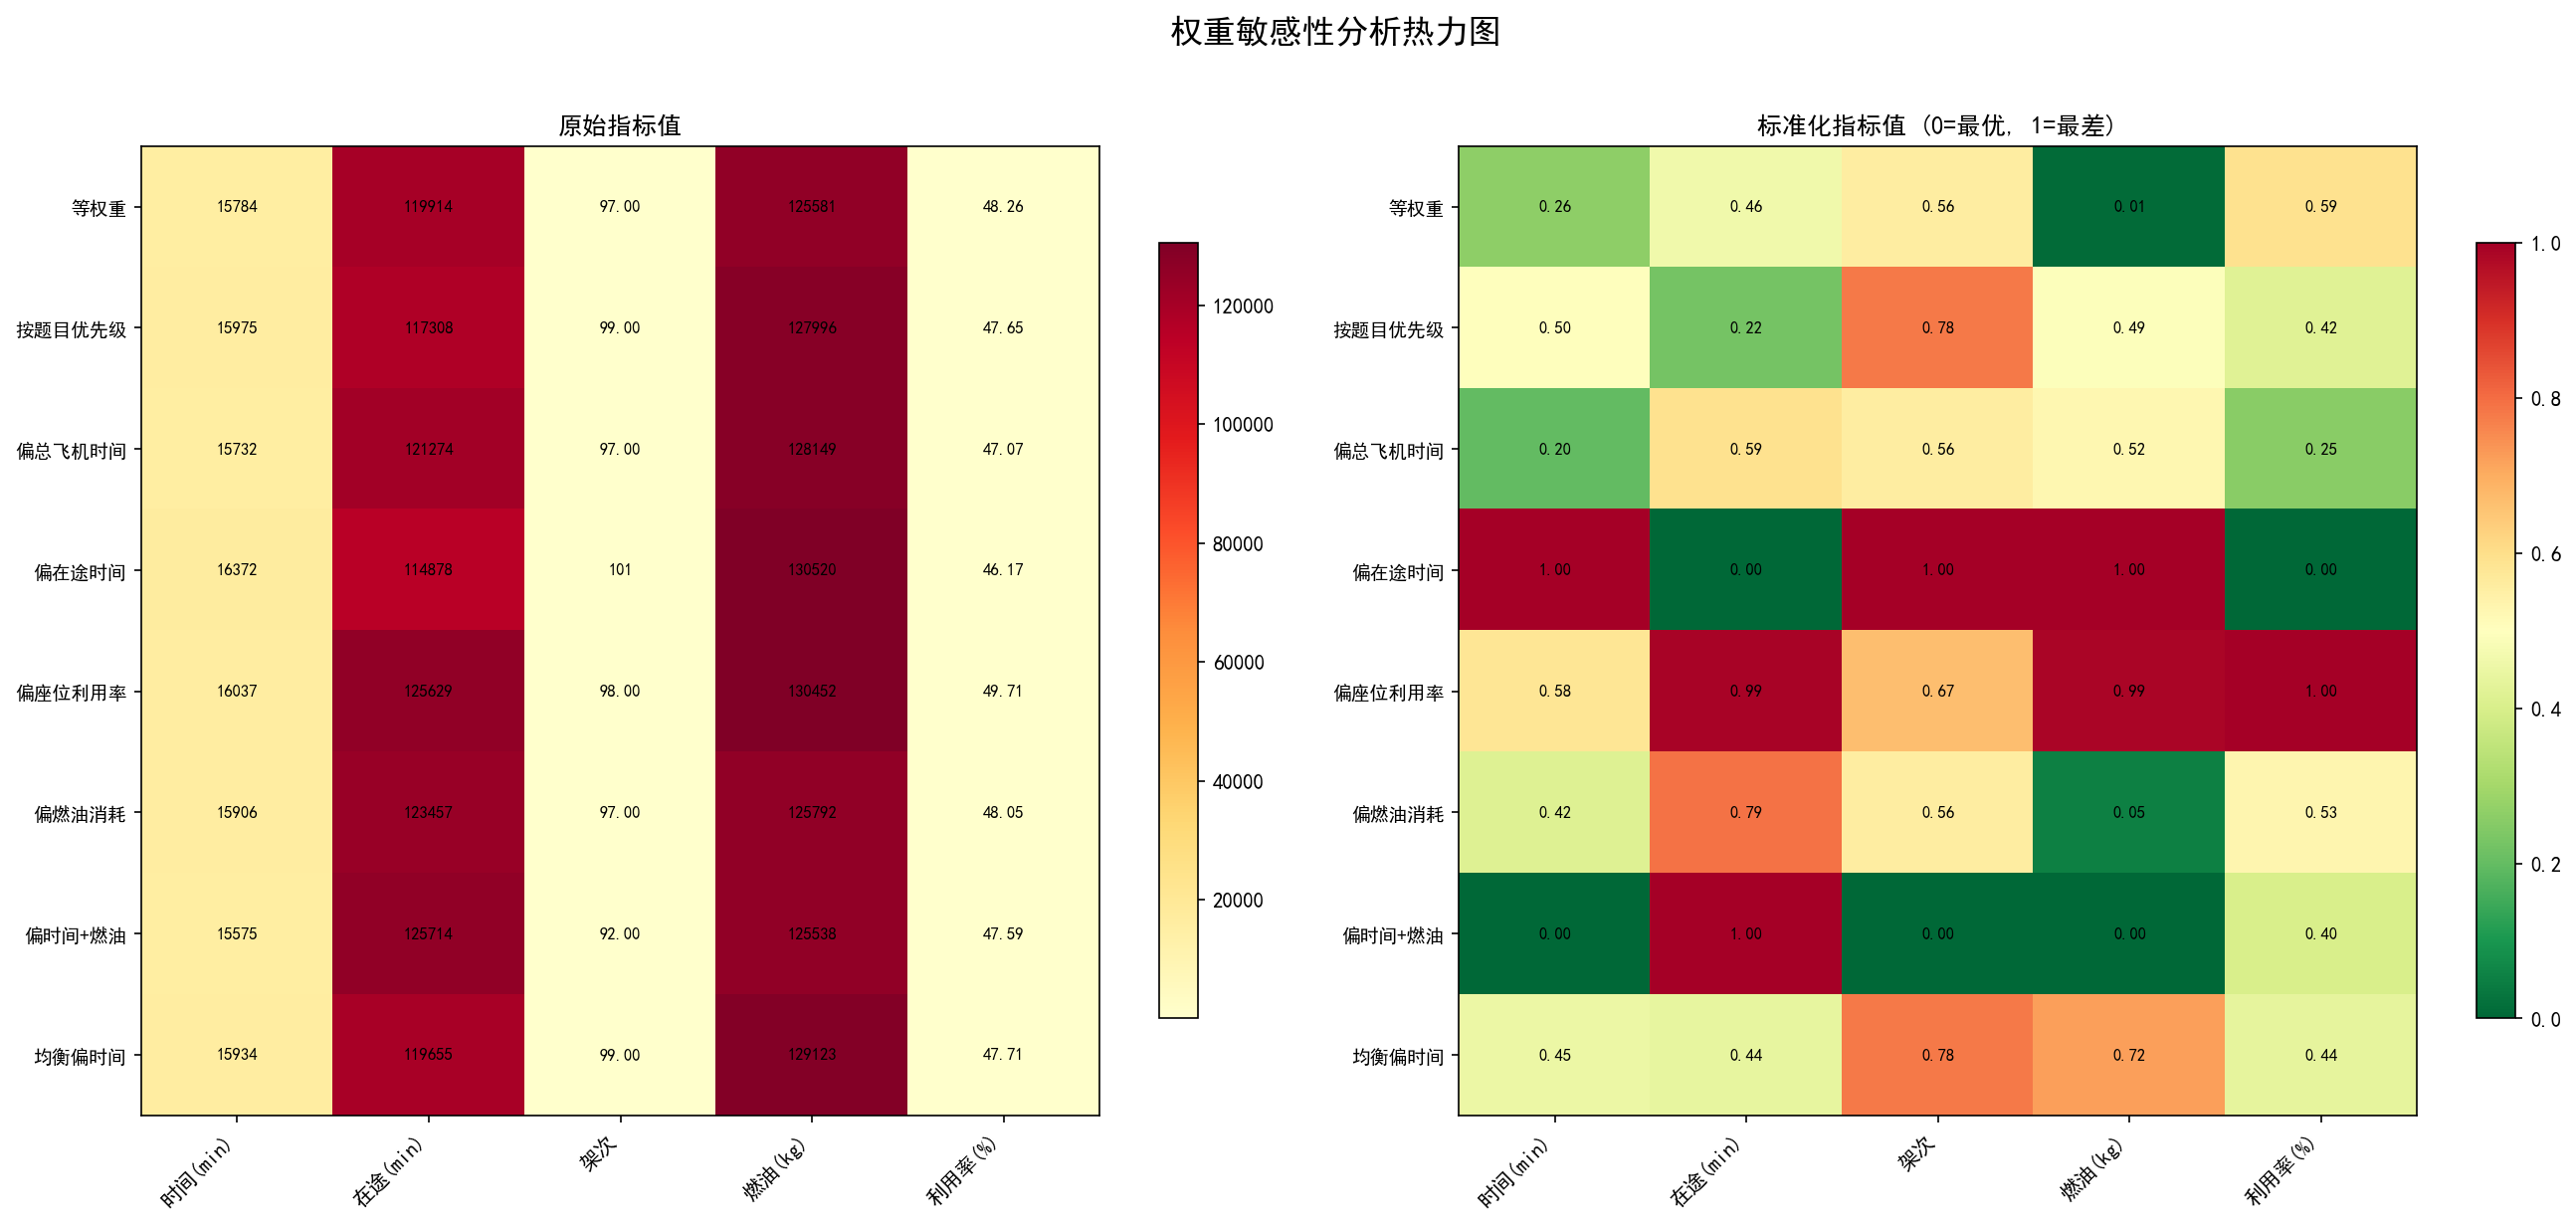
\includegraphics[width=0.85\textwidth]{../figures/Problem3/extra/G6_weight_sensitivity_heatmap.png}
\caption{权重敏感性热力图（8 方案 $\times$ 5 指标）}
\label{fig:weight_sensitivity}
\end{figure}

\subsection{最优性间隙与计算瓶颈}

问题三的拉格朗日下界分析表明，最优性间隙为 80.30\%（COPT 内置下界）。这一间隙主要源于 MIP 求解器在 90 s 时限内的计算能力限制，而非模型缺陷。进阶方法探索（C7 聚类、C8 列生成）的实验结果进一步印证了这一判断：C7 因时间窗过宽而失效，C8 改善有限（在途 $-4.36\%$）恰因 MIP 间隙过高导致求解器无法充分利用更大的路径池。

